\section{Richard-Germay-Detournay Family of Bit Model}
%\section{RGD Family of Models}
\label{ch:rgdmodels}

\subsection{Introduction}
While the current project focuses on drill string models, it is natural to couple a string model with a bit model. The Richard-Germay-Detournay family of bit models (RGD models) represents theoretical bit-rock interactions. They use a more sophisticated approach than many bit models and are, therefore, of interest. The RGD model is developed by Richard et al., 2007\ \cite{ref:richard2007a}, which simulates coupled axial and torsional vibration mode through bit-rock interaction. The model has been applied to numerous drill-string models to model bit-rock interactions.

\subsection{RGD Model}
The model combines governing equations of motions (axial and torsional) with bit-rock interface law which leads to a state-dependent delay system. Also, the model takes into account the loss of contact at wearflat/rock interface caused by axial vibration of the bit through a discontinuous boundary conditions. A brief description of the mathematical background is shown in \figurename~\ref{figure_RGD_Summary}.
\begin{figure}
  \centering
  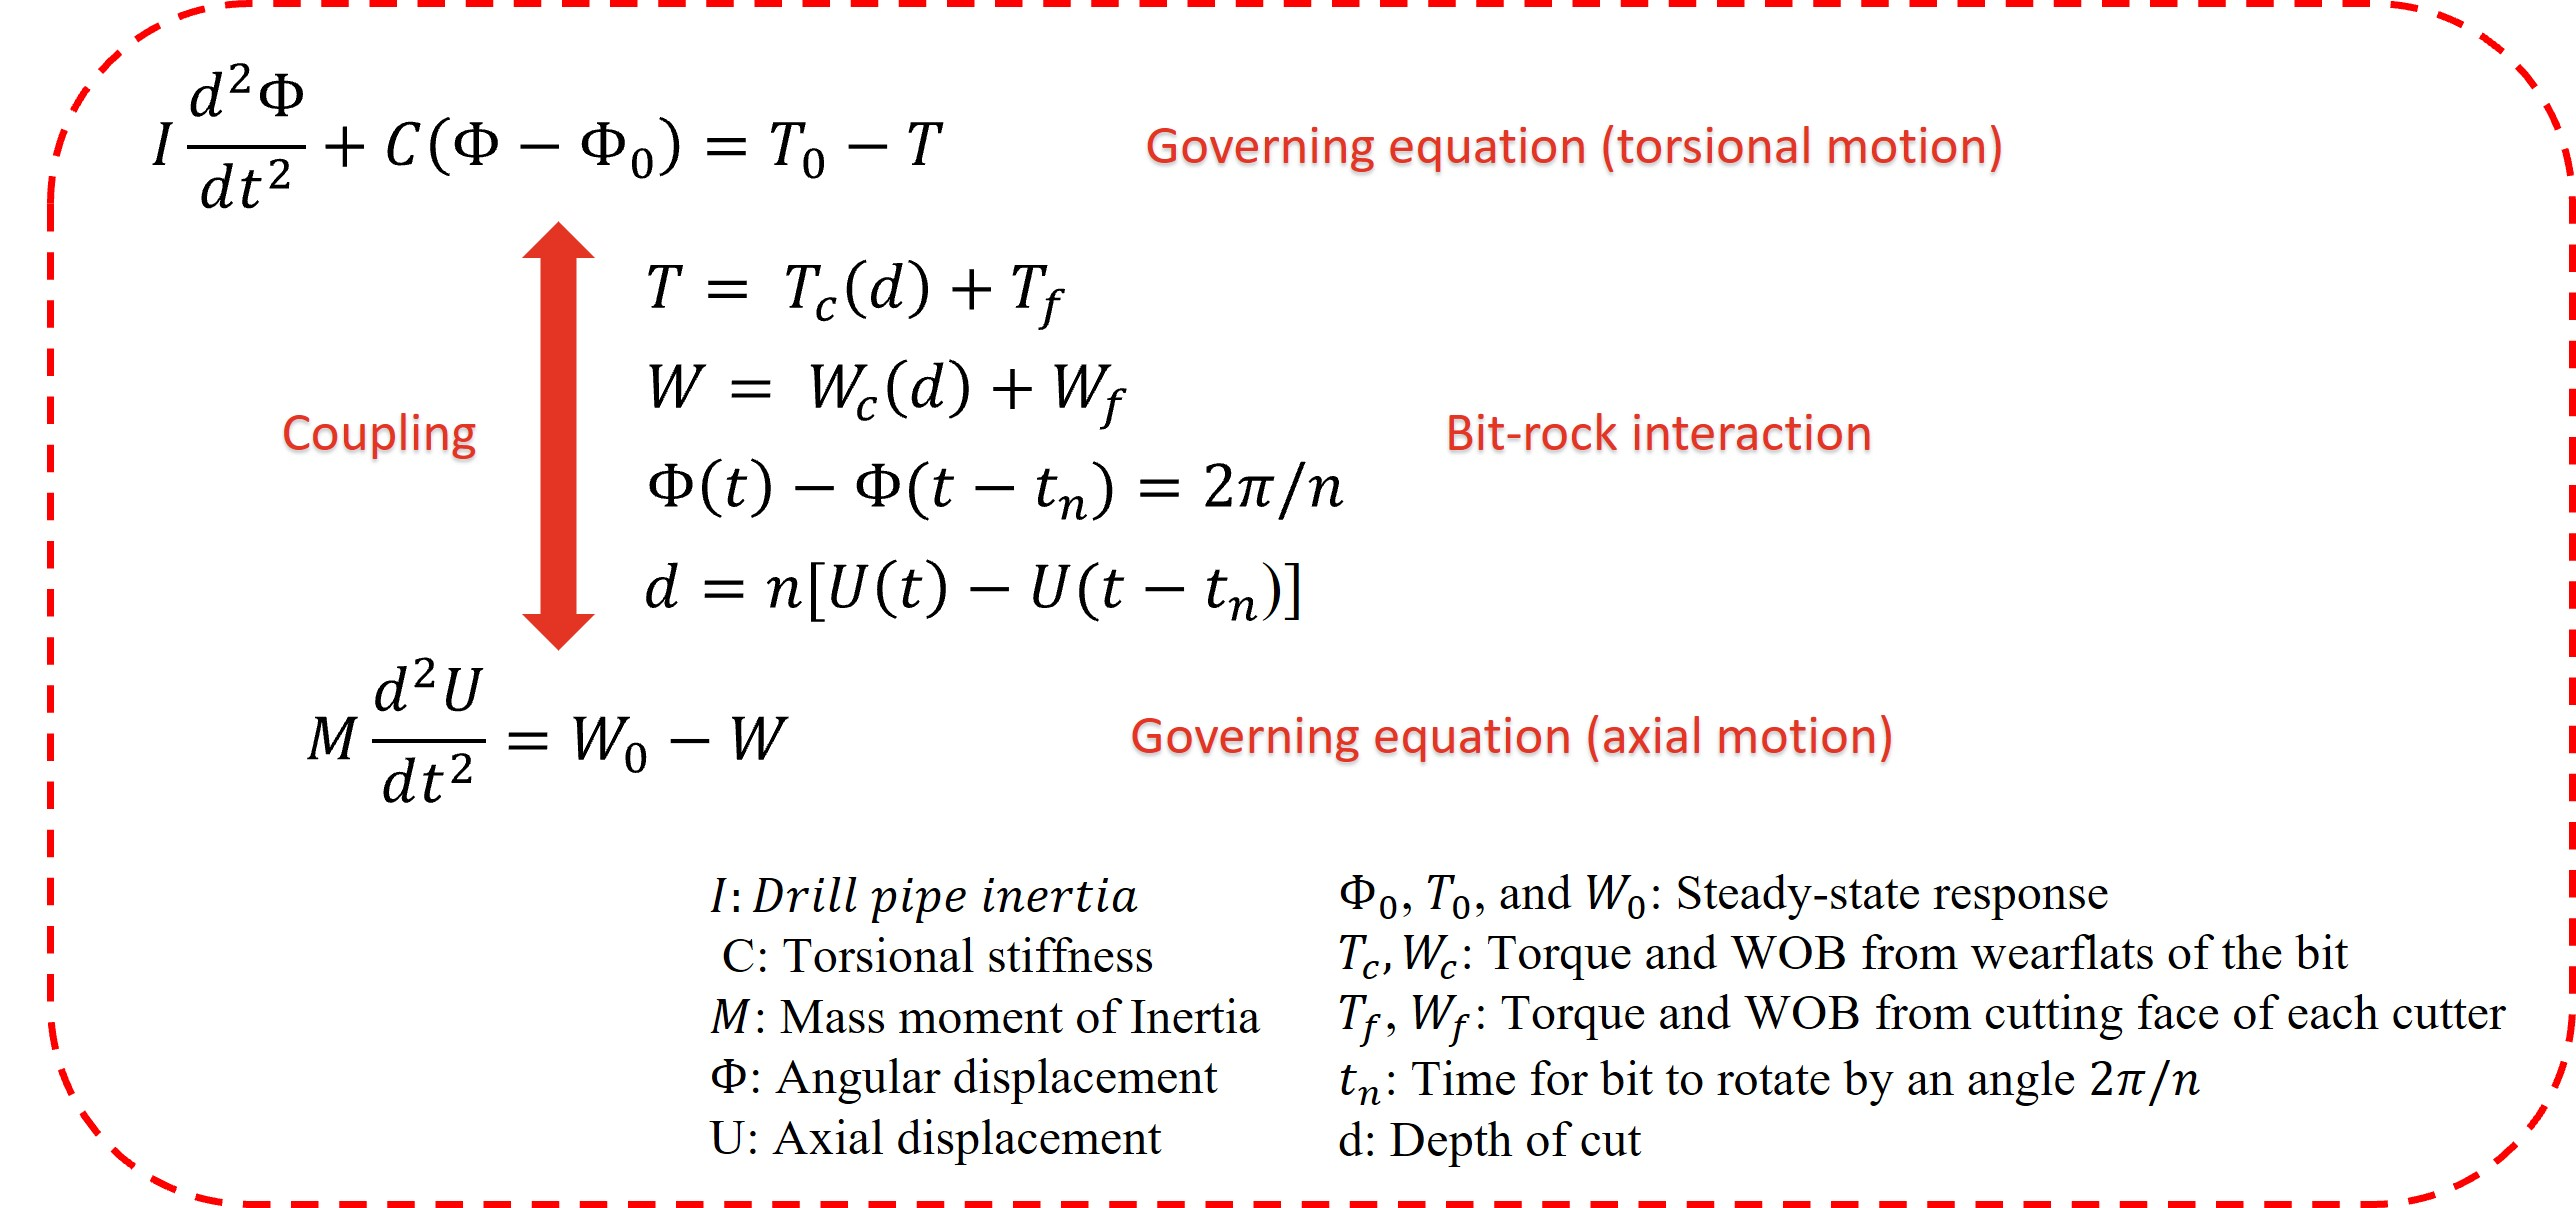
\includegraphics[width=5in]{RGD_summary}
  \caption[Mathematical description of RGD model]{Mathematical description of RGD model.}\label{figure_RGD_Summary}
\end{figure}
The model uses a 2 DOF system with torsional and axial modes coupled by bit-rock interaction model by the depth of cut. \needsclarification{} Moreover, functions $T_c$, $T_f$, $W_C$ and $W_f$ \reviewcomment{Define parameters.} are defined with respect to the drilling regime which reflects the discontinuous boundary conditions. \needsclarification{} The drilling regimes are classified as 1.\ cutting ($\omega>0, d>0$), 2.\ sticking ($\omega=0, d>0$) 3.\ sliding ($\omega>0, d=0$), 4.\ and off-bottom ($\omega>0, d<0$). \reviewcomment{Are these intended to be ordered or numbered?}

The base assumptions of the model are:
\begin{bulletedlist}
	\item Constant angular velocity and upward force at the top of the drill string
	\item A vertical borehole
	\item No lateral motion of the bit
	\item Most of the energy dissipation occurs at the bit-rock interface
\end{bulletedlist}
Because it assumes the energy dissipation is at the bit-rock interface, additional damping parameters are not used.

The self-excited vibration was demonstrated and the model was also validated with laboratory tests. \needsclarification[Wording?]

Since the model is a for the bit and not the drill string model, and it is limited to vertical well, it was not selected for this project. Moreover, because of the limited degrees of freedom, the model was not able to capture stick-slip occurrence at a frequency higher than the first torsional mode. \reviewcomment{Stick-slip is generally at the fundamental frequency.}

\subsection{Extended RGD Model}
Numerous drill string models benchmarked RGD model for bit-rock interactions. \figurename~\ref{model_develop_figure} illustrates the development of the RGD model.
\begin{figure}
  \centering
  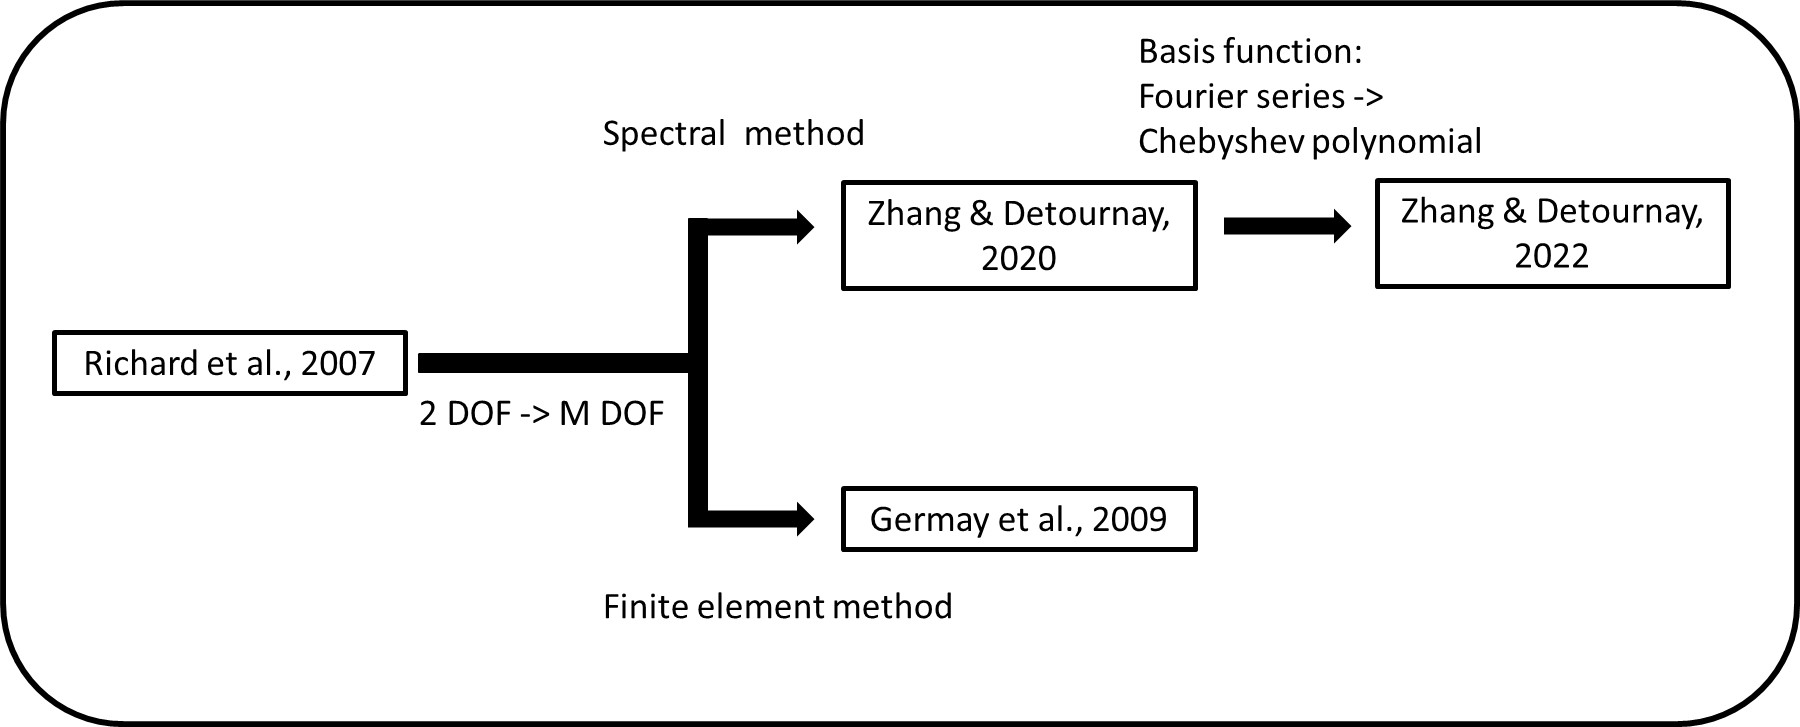
\includegraphics[width=5in]{ModelDevelop}
  \caption[RGD model development]{RGD model development.}\label{model_develop_figure}
\end{figure} 
Germay increased DOF \reviewcomment{Now this is becoming a drill string \emph{and} bit model.  We need to clarify the wording.} of the model by discretizing the drill string and applying the finite element method \referencename~\cite{ref:germay2009a}. This model was able to simulate the stick \reviewcomment{Full stick?} phase that occurred by vibration higher than the first natural torsional frequency. Similarly, Zhang increased the DOF of the model by implementing the spectral method and further improved the computational efficiency by applying Chebyshev polynomial as a basis function \referencename~\cite{ref:zhang2020a}. The model was able to simulate axial and torsional vibrations, including stick-slip events, with enhanced computation efficiency compared to the FEM approach in a geometrically simple structure. The source code was not provided, therefore;\reviewcomment{Semi colon} we could not test for this project. \reviewcomment{Source code for one or both?} However, these models can be good candidates for further study. The source code of the 2 DOF RGD bit model, applying the spectral method is provided, and mathematical details based on the code can be seen in \appendixname~\ref{ap:rgbworkflow}. \reviewcomment{Appendix is for spectral method?} 